\documentclass[tikz,border=3mm]{standalone}
\usetikzlibrary{arrows.meta, positioning, shapes.geometric, fit}

\begin{document}
\sffamily
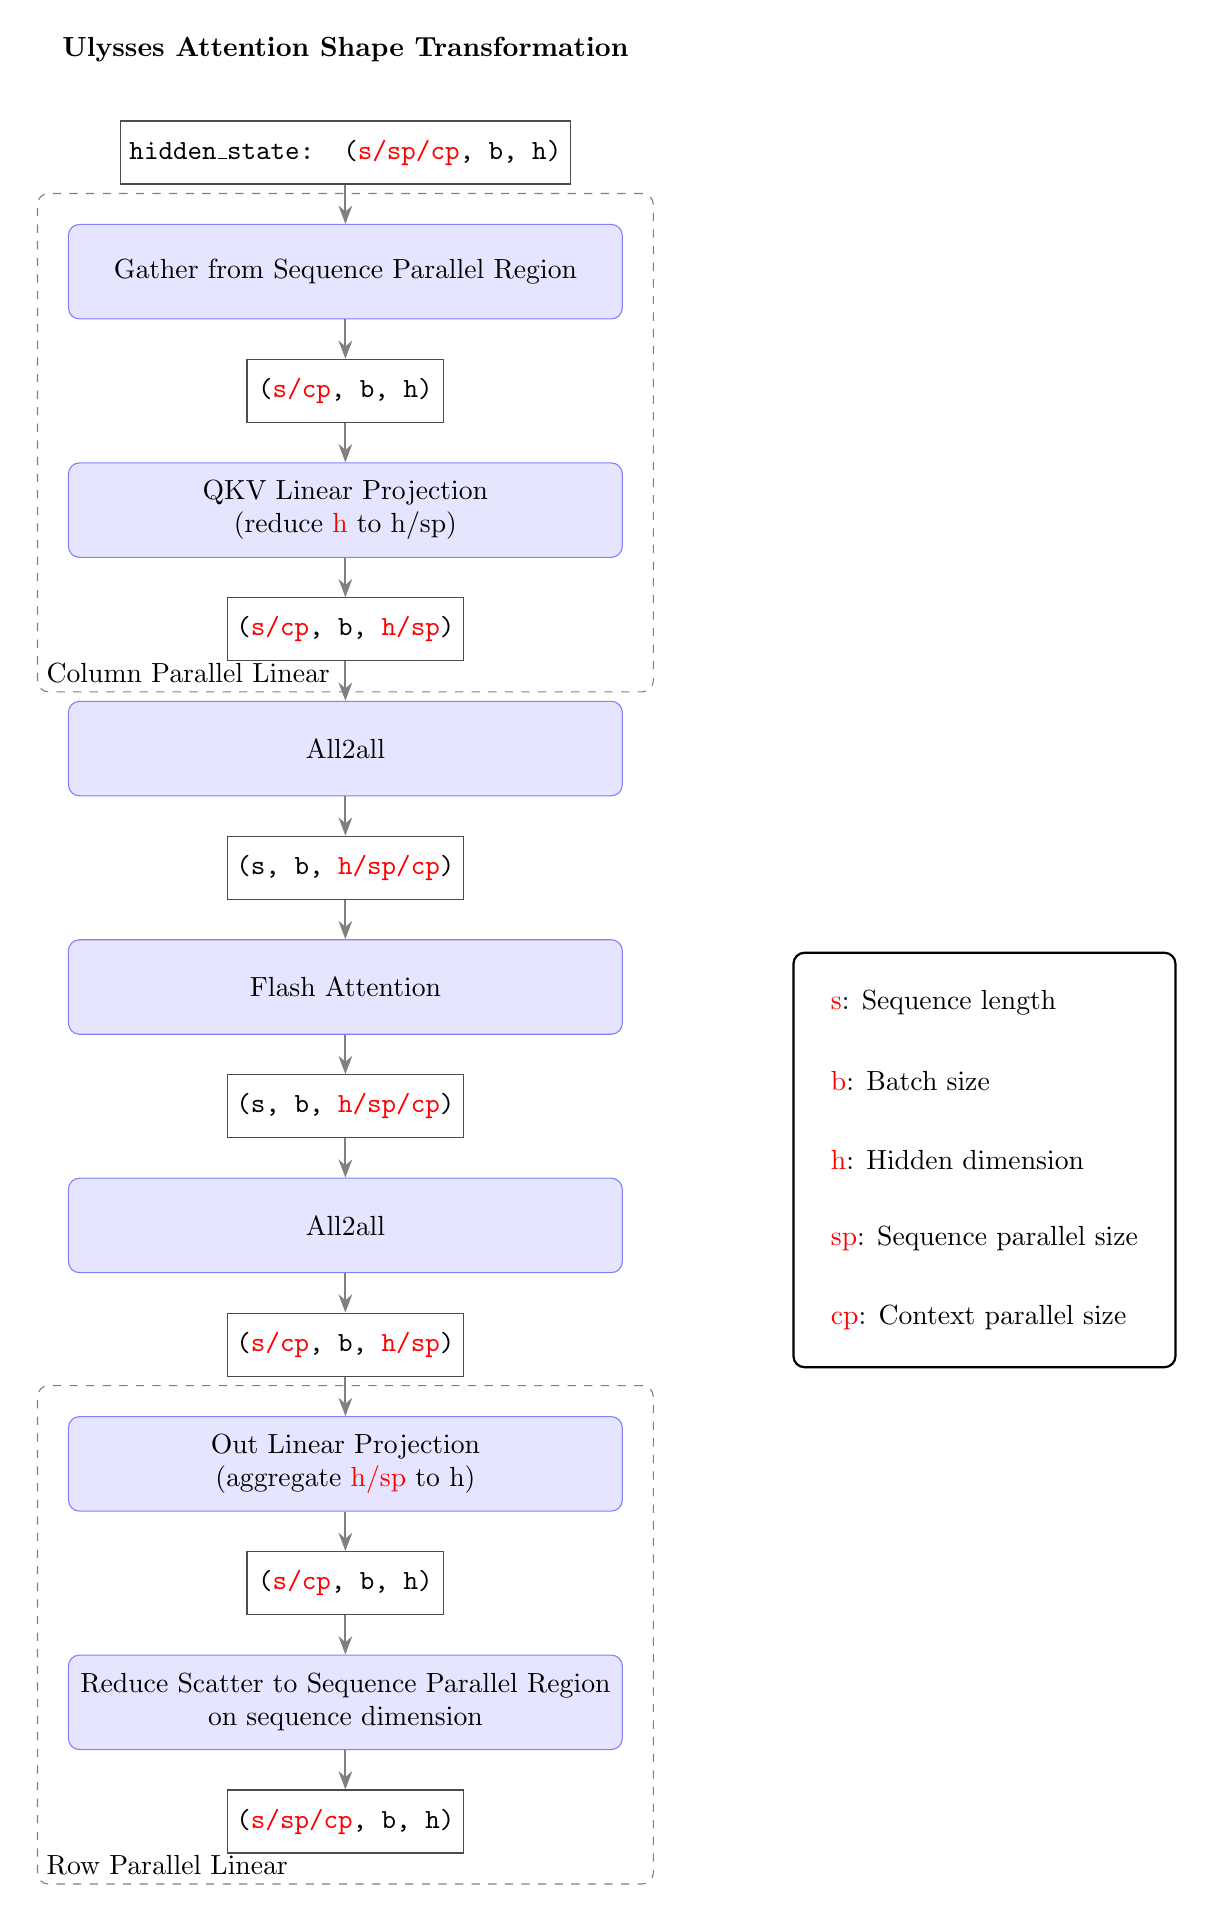
\begin{tikzpicture}[
    node distance=5mm,
    operation/.style={rectangle, draw=blue!50, fill=blue!10, rounded corners, minimum width=7cm, minimum height=1.2cm, text width=6.8cm, align=center},
    shapebox/.style={rectangle, draw=black!70, fill=white, minimum width=2.5cm, minimum height=0.8cm, font=\ttfamily},
    arrow/.style={-Stealth, thick, draw=black!50},
    groupbox/.style={draw=black!50, dashed, rounded corners, inner sep=11pt},
    outerbox/.style={},
    legendbox/.style={draw=black, thick, rounded corners, inner sep=10pt}
]

% 初始输入
\node[shapebox] (input) {hidden\_state: (\textcolor{red}{s/sp/cp}, b, h)};

% AG
\node[operation, below=of input] (ag) {Gather from Sequence Parallel Region};
\node[shapebox, below=of ag] (ag-output) {(\textcolor{red}{s/cp}, b, h)};

% proj
\node[operation, below=of ag-output] (proj) {QKV Linear Projection \\ (reduce \textcolor{red}{h} to h/sp)};
\node[shapebox, below=of proj] (proj-output) {(\textcolor{red}{s/cp}, b, \textcolor{red}{h/sp})};

% a2a
\node[operation, below=of proj-output] (a2a) {All2all};
\node[shapebox, below=of a2a] (a2a-output) {(s, b, \textcolor{red}{h/sp/cp})};

% fa
\node[operation, below=of a2a-output] (fa) {Flash Attention};
\node[shapebox, below=of fa] (fa-output) {(s, b, \textcolor{red}{h/sp/cp})};

% a2a2
\node[operation, below=of fa-output] (a2a2) {All2all};
\node[shapebox, below=of a2a2] (a2a2-output) {(\textcolor{red}{s/cp}, b, \textcolor{red}{h/sp})};

% oproj
\node[operation, below=of a2a2-output] (oproj) {Out Linear Projection \\ (aggregate \textcolor{red}{h/sp} to h)};
\node[shapebox, below=of oproj] (oproj-output) {(\textcolor{red}{s/cp}, b, h)};

% rs
\node[operation, below=of oproj-output] (rs) {Reduce Scatter to Sequence Parallel Region \\ on sequence dimension};
\node[shapebox, below=of rs] (rs-output) {(\textcolor{red}{s/sp/cp}, b, h)};

% 连接箭头
\draw[arrow] (input) -- (ag);
\draw[arrow] (ag) -- (ag-output);
\draw[arrow] (ag-output) -- (proj);
\draw[arrow] (proj) -- (proj-output);
\draw[arrow] (proj-output) -- (a2a);
\draw[arrow] (a2a) -- (a2a-output);
\draw[arrow] (a2a-output) -- (fa);
\draw[arrow] (fa) -- (fa-output);
\draw[arrow] (fa-output) -- (a2a2);
\draw[arrow] (a2a2) -- (a2a2-output);
\draw[arrow] (a2a2-output) -- (oproj);
\draw[arrow] (oproj) -- (oproj-output);
\draw[arrow] (oproj-output) -- (rs);
\draw[arrow] (rs) -- (rs-output);

% 添加分组框
\node[groupbox, fit=(ag) (ag-output) (proj) (proj-output), label={[anchor=south west]south west:Column Parallel Linear}] (agprojbox) {};
\node[groupbox, fit=(oproj) (oproj-output) (rs) (rs-output), label={[anchor=south west]south west:Row Parallel Linear}] (oprojrsbox) {};

% 添加外框
\node[outerbox, fit=(input) (rs-output) (agprojbox) (oprojrsbox)] (outerbox) {};

% 维度说明
\node[anchor=west] at ([xshift=2cm]outerbox.east) (legend1) {\textcolor{red}{s}: Sequence length};
\node[anchor=west] at ([xshift=2cm]outerbox.east) [yshift=-1cm] (legend2) {\textcolor{red}{b}: Batch size};
\node[anchor=west] at ([xshift=2cm]outerbox.east) [yshift=-2cm] (legend3) {\textcolor{red}{h}: Hidden dimension};
\node[anchor=west] at ([xshift=2cm]outerbox.east) [yshift=-3cm] (legend4) {\textcolor{red}{sp}: Sequence parallel size};
\node[anchor=west] at ([xshift=2cm]outerbox.east) [yshift=-4cm] (legend5) {\textcolor{red}{cp}: Context parallel size};
\node[legendbox, fit=(legend1) (legend2) (legend3) (legend4) (legend5)] {};

% 标题
\node[above=5mm of outerbox, font=\bfseries] {Ulysses Attention Shape Transformation};
\end{tikzpicture}
\end{document}